\documentclass[1p]{elsarticle_modified}
%\bibliographystyle{elsarticle-num}

%\usepackage[colorlinks]{hyperref}
%\usepackage{abbrmath_seonhwa} %\Abb, \Ascr, \Acal ,\Abf, \Afrak
\usepackage{amsfonts}
\usepackage{amssymb}
\usepackage{amsmath}
\usepackage{amsthm}
\usepackage{scalefnt}
\usepackage{amsbsy}
\usepackage{kotex}
\usepackage{caption}
\usepackage{subfig}
\usepackage{color}
\usepackage{graphicx}
\usepackage{xcolor} %% white, black, red, green, blue, cyan, magenta, yellow
\usepackage{float}
\usepackage{setspace}
\usepackage{hyperref}

\usepackage{tikz}
\usetikzlibrary{arrows}

\usepackage{multirow}
\usepackage{array} % fixed length table
\usepackage{hhline}

%%%%%%%%%%%%%%%%%%%%%
\makeatletter
\renewcommand*\env@matrix[1][\arraystretch]{%
	\edef\arraystretch{#1}%
	\hskip -\arraycolsep
	\let\@ifnextchar\new@ifnextchar
	\array{*\c@MaxMatrixCols c}}
\makeatother %https://tex.stackexchange.com/questions/14071/how-can-i-increase-the-line-spacing-in-a-matrix
%%%%%%%%%%%%%%%

\usepackage[normalem]{ulem}

\newcommand{\msout}[1]{\ifmmode\text{\sout{\ensuremath{#1}}}\else\sout{#1}\fi}
%SOURCE: \msout is \stkout macro in https://tex.stackexchange.com/questions/20609/strikeout-in-math-mode

\newcommand{\cancel}[1]{
	\ifmmode
	{\color{red}\msout{#1}}
	\else
	{\color{red}\sout{#1}}
	\fi
}

\newcommand{\add}[1]{
	{\color{blue}\uwave{#1}}
}

\newcommand{\replace}[2]{
	\ifmmode
	{\color{red}\msout{#1}}{\color{blue}\uwave{#2}}
	\else
	{\color{red}\sout{#1}}{\color{blue}\uwave{#2}}
	\fi
}

\newcommand{\Sol}{\mathcal{S}} %segment
\newcommand{\D}{D} %diagram
\newcommand{\A}{\mathcal{A}} %arc


%%%%%%%%%%%%%%%%%%%%%%%%%%%%%5 test

\def\sl{\operatorname{\textup{SL}}(2,\Cbb)}
\def\psl{\operatorname{\textup{PSL}}(2,\Cbb)}
\def\quan{\mkern 1mu \triangleright \mkern 1mu}

\theoremstyle{definition}
\newtheorem{thm}{Theorem}[section]
\newtheorem{prop}[thm]{Proposition}
\newtheorem{lem}[thm]{Lemma}
\newtheorem{ques}[thm]{Question}
\newtheorem{cor}[thm]{Corollary}
\newtheorem{defn}[thm]{Definition}
\newtheorem{exam}[thm]{Example}
\newtheorem{rmk}[thm]{Remark}
\newtheorem{alg}[thm]{Algorithm}

\newcommand{\I}{\sqrt{-1}}
\begin{document}

%\begin{frontmatter}
%
%\title{Boundary parabolic representations of knots up to 8 crossings}
%
%%% Group authors per affiliation:
%\author{Yunhi Cho} 
%\address{Department of Mathematics, University of Seoul, Seoul, Korea}
%\ead{yhcho@uos.ac.kr}
%
%
%\author{Seonhwa Kim} %\fnref{s_kim}}
%\address{Center for Geometry and Physics, Institute for Basic Science, Pohang, 37673, Korea}
%\ead{ryeona17@ibs.re.kr}
%
%\author{Hyuk Kim}
%\address{Department of Mathematical Sciences, Seoul National University, Seoul 08826, Korea}
%\ead{hyukkim@snu.ac.kr}
%
%\author{Seokbeom Yoon}
%\address{Department of Mathematical Sciences, Seoul National University, Seoul, 08826,  Korea}
%\ead{sbyoon15@snu.ac.kr}
%
%\begin{abstract}
%We find all boundary parabolic representation of knots up to 8 crossings.
%
%\end{abstract}
%\begin{keyword}
%    \MSC[2010] 57M25 
%\end{keyword}
%
%\end{frontmatter}

%\linenumbers
%\tableofcontents
%
\newcommand\colored[1]{\textcolor{white}{\rule[-0.35ex]{0.8em}{1.4ex}}\kern-0.8em\color{red} #1}%
%\newcommand\colored[1]{\textcolor{white}{ #1}\kern-2.17ex	\textcolor{white}{ #1}\kern-1.81ex	\textcolor{white}{ #1}\kern-2.15ex\color{red}#1	}

{\Large $\underline{12n_{0562}~(K12n_{0562})}$}

\setlength{\tabcolsep}{10pt}
\renewcommand{\arraystretch}{1.6}
\vspace{1cm}\begin{tabular}{m{100pt}>{\centering\arraybackslash}m{274pt}}
\multirow{5}{120pt}{
	\centering
	\includegraphics[width=112pt]{../../../GIT/diagram.site/Diagrams/png/2651_12n_0562.png}\\
\ \ \ A knot diagram\footnotemark}&
\allowdisplaybreaks
\textbf{Linearized knot diagam} \\
\cline{2-2}
 &
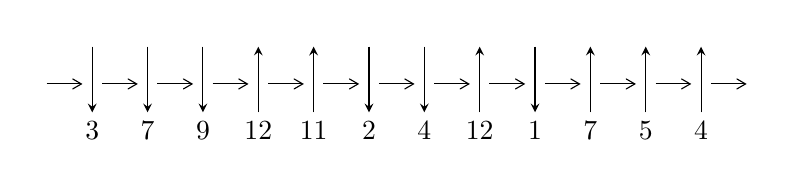
\begin{tikzpicture}[x=20pt, y=17pt]
	% nodes
	\node (C0) at (0, 0) {};
	\node (C1) at (1, 0) {};
	\node (C1U) at (1, +1) {};
	\node (C1D) at (1, -1) {3};

	\node (C2) at (2, 0) {};
	\node (C2U) at (2, +1) {};
	\node (C2D) at (2, -1) {7};

	\node (C3) at (3, 0) {};
	\node (C3U) at (3, +1) {};
	\node (C3D) at (3, -1) {9};

	\node (C4) at (4, 0) {};
	\node (C4U) at (4, +1) {};
	\node (C4D) at (4, -1) {12};

	\node (C5) at (5, 0) {};
	\node (C5U) at (5, +1) {};
	\node (C5D) at (5, -1) {11};

	\node (C6) at (6, 0) {};
	\node (C6U) at (6, +1) {};
	\node (C6D) at (6, -1) {2};

	\node (C7) at (7, 0) {};
	\node (C7U) at (7, +1) {};
	\node (C7D) at (7, -1) {4};

	\node (C8) at (8, 0) {};
	\node (C8U) at (8, +1) {};
	\node (C8D) at (8, -1) {12};

	\node (C9) at (9, 0) {};
	\node (C9U) at (9, +1) {};
	\node (C9D) at (9, -1) {1};

	\node (C10) at (10, 0) {};
	\node (C10U) at (10, +1) {};
	\node (C10D) at (10, -1) {7};

	\node (C11) at (11, 0) {};
	\node (C11U) at (11, +1) {};
	\node (C11D) at (11, -1) {5};

	\node (C12) at (12, 0) {};
	\node (C12U) at (12, +1) {};
	\node (C12D) at (12, -1) {4};
	\node (C13) at (13, 0) {};

	% arrows
	\draw[->,>={angle 60}]
	(C0) edge (C1) (C1) edge (C2) (C2) edge (C3) (C3) edge (C4) (C4) edge (C5) (C5) edge (C6) (C6) edge (C7) (C7) edge (C8) (C8) edge (C9) (C9) edge (C10) (C10) edge (C11) (C11) edge (C12) (C12) edge (C13) ;	\draw[->,>=stealth]
	(C1U) edge (C1D) (C2U) edge (C2D) (C3U) edge (C3D) (C4D) edge (C4U) (C5D) edge (C5U) (C6U) edge (C6D) (C7U) edge (C7D) (C8D) edge (C8U) (C9U) edge (C9D) (C10D) edge (C10U) (C11D) edge (C11U) (C12D) edge (C12U) ;
	\end{tikzpicture} \\
\hhline{~~} \\& 
\textbf{Solving Sequence} \\ \cline{2-2} 
 &
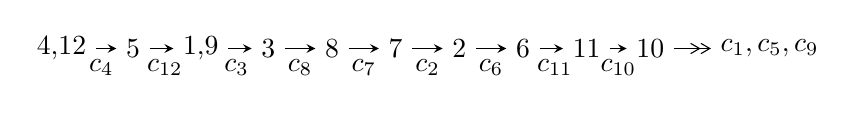
\begin{tikzpicture}[x=23pt, y=7pt]
	% node
	\node (A0) at (-1/8, 0) {4,12};
	\node (A1) at (1, 0) {5};
	\node (A2) at (33/16, 0) {1,9};
	\node (A3) at (25/8, 0) {3};
	\node (A4) at (33/8, 0) {8};
	\node (A5) at (41/8, 0) {7};
	\node (A6) at (49/8, 0) {2};
	\node (A7) at (57/8, 0) {6};
	\node (A8) at (65/8, 0) {11};
	\node (A9) at (73/8, 0) {10};
	\node (C1) at (1/2, -1) {$c_{4}$};
	\node (C2) at (3/2, -1) {$c_{12}$};
	\node (C3) at (21/8, -1) {$c_{3}$};
	\node (C4) at (29/8, -1) {$c_{8}$};
	\node (C5) at (37/8, -1) {$c_{7}$};
	\node (C6) at (45/8, -1) {$c_{2}$};
	\node (C7) at (53/8, -1) {$c_{6}$};
	\node (C8) at (61/8, -1) {$c_{11}$};
	\node (C9) at (69/8, -1) {$c_{10}$};
	\node (A10) at (11, 0) {$c_{1},c_{5},c_{9}$};

	% edge
	\draw[->,>=stealth]	
	(A0) edge (A1) (A1) edge (A2) (A2) edge (A3) (A3) edge (A4) (A4) edge (A5) (A5) edge (A6) (A6) edge (A7) (A7) edge (A8) (A8) edge (A9) ;
	\draw[->>,>={angle 60}]	
	(A9) edge (A10);
\end{tikzpicture} \\ 

\end{tabular} \\

\footnotetext{
The image of knot diagram is generated by the software ``\textbf{Draw programme}" developed by Andrew Bartholomew(\url{http://www.layer8.co.uk/maths/draw/index.htm\#Running-draw}), where we modified some parts for our purpose(\url{https://github.com/CATsTAILs/LinksPainter}).
}\phantom \\ \newline 
\centering \textbf{Ideals for irreducible components\footnotemark of $X_{\text{par}}$} 
 
\begin{align*}
I^u_{1}&=\langle 
-1863653922 u^{24}-2022363077 u^{23}+\cdots+3360966496 b+12865105183,\\
\phantom{I^u_{1}}&\phantom{= \langle  }1528807327 u^{24}+2234282167 u^{23}+\cdots+3360966496 a+6708798419,\;u^{25}+u^{24}+\cdots-13 u+1\rangle \\
I^u_{2}&=\langle 
- u^3+b-2 u,\;u^2 a+a^2+u^2+2 a+3,\;u^4+3 u^2+1\rangle \\
\\
\end{align*}
\raggedright * 2 irreducible components of $\dim_{\mathbb{C}}=0$, with total 33 representations.\\
\footnotetext{All coefficients of polynomials are rational numbers. But the coefficients are sometimes approximated in decimal forms when there is not enough margin.}
\newpage
\renewcommand{\arraystretch}{1}
\centering \section*{I. $I^u_{1}= \langle -1.86\times10^{9} u^{24}-2.02\times10^{9} u^{23}+\cdots+3.36\times10^{9} b+1.29\times10^{10},\;1.53\times10^{9} u^{24}+2.23\times10^{9} u^{23}+\cdots+3.36\times10^{9} a+6.71\times10^{9},\;u^{25}+u^{24}+\cdots-13 u+1 \rangle$}
\flushleft \textbf{(i) Arc colorings}\\
\begin{tabular}{m{7pt} m{180pt} m{7pt} m{180pt} }
\flushright $a_{4}=$&$\begin{pmatrix}1\\0\end{pmatrix}$ \\
\flushright $a_{12}=$&$\begin{pmatrix}0\\u\end{pmatrix}$ \\
\flushright $a_{5}=$&$\begin{pmatrix}1\\- u^2\end{pmatrix}$ \\
\flushright $a_{1}=$&$\begin{pmatrix}u\\u\end{pmatrix}$ \\
\flushright $a_{9}=$&$\begin{pmatrix}-0.454871 u^{24}-0.664774 u^{23}+\cdots-25.1625 u-1.99609\\0.554499 u^{24}+0.601721 u^{23}+\cdots+24.9344 u-3.82780\end{pmatrix}$ \\
\flushright $a_{3}=$&$\begin{pmatrix}3.46960 u^{24}+3.91721 u^{23}+\cdots+154.960 u-24.4260\\0.0868909 u^{24}+0.140131 u^{23}+\cdots+2.56515 u+0.501418\end{pmatrix}$ \\
\flushright $a_{8}=$&$\begin{pmatrix}-0.454871 u^{24}-0.664774 u^{23}+\cdots-25.1625 u-1.99609\\0.508672 u^{24}+0.570274 u^{23}+\cdots+22.6605 u-3.61790\end{pmatrix}$ \\
\flushright $a_{7}=$&$\begin{pmatrix}0.0538011 u^{24}-0.0944999 u^{23}+\cdots-2.50201 u-5.61399\\0.508672 u^{24}+0.570274 u^{23}+\cdots+22.6605 u-3.61790\end{pmatrix}$ \\
\flushright $a_{2}=$&$\begin{pmatrix}1.70781 u^{24}+1.96070 u^{23}+\cdots+78.9836 u-7.58147\\-0.391234 u^{24}-0.397877 u^{23}+\cdots-17.0453 u+3.25795\end{pmatrix}$ \\
\flushright $a_{6}=$&$\begin{pmatrix}- u^2-1\\u^4+2 u^2\end{pmatrix}$ \\
\flushright $a_{11}=$&$\begin{pmatrix}- u\\u^3+u\end{pmatrix}$ \\
\flushright $a_{10}=$&$\begin{pmatrix}-0.491571 u^{24}-0.694228 u^{23}+\cdots-27.4957 u-1.73897\\0.517800 u^{24}+0.572267 u^{23}+\cdots+22.6011 u-3.57068\end{pmatrix}$\\&\end{tabular}
\flushleft \textbf{(ii) Obstruction class $= -1$}\\~\\
\flushleft \textbf{(iii) Cusp Shapes $= -\frac{2040219475}{840241624} u^{24}-\frac{4044991761}{1680483248} u^{23}+\cdots-\frac{48458587153}{420120812} u+\frac{40726820499}{1680483248}$}\\~\\
\newpage\renewcommand{\arraystretch}{1}
\flushleft \textbf{(iv) u-Polynomials at the component}\newline \\
\begin{tabular}{m{50pt}|m{274pt}}
Crossings & \hspace{64pt}u-Polynomials at each crossing \\
\hline $$\begin{aligned}c_{1}\end{aligned}$$&$\begin{aligned}
&u^{25}+17 u^{24}+\cdots-99 u+25
\end{aligned}$\\
\hline $$\begin{aligned}c_{2},c_{6}\end{aligned}$$&$\begin{aligned}
&u^{25}- u^{24}+\cdots- u+5
\end{aligned}$\\
\hline $$\begin{aligned}c_{3}\end{aligned}$$&$\begin{aligned}
&u^{25}- u^{24}+\cdots+4 u+4
\end{aligned}$\\
\hline $$\begin{aligned}c_{4},c_{5},c_{11}\\c_{12}\end{aligned}$$&$\begin{aligned}
&u^{25}+u^{24}+\cdots-13 u+1
\end{aligned}$\\
\hline $$\begin{aligned}c_{7}\end{aligned}$$&$\begin{aligned}
&u^{25}+3 u^{24}+\cdots-64 u+16
\end{aligned}$\\
\hline $$\begin{aligned}c_{8}\end{aligned}$$&$\begin{aligned}
&u^{25}-3 u^{24}+\cdots+u-5
\end{aligned}$\\
\hline $$\begin{aligned}c_{9}\end{aligned}$$&$\begin{aligned}
&u^{25}+3 u^{24}+\cdots-508 u-284
\end{aligned}$\\
\hline $$\begin{aligned}c_{10}\end{aligned}$$&$\begin{aligned}
&u^{25}-3 u^{24}+\cdots-88 u+16
\end{aligned}$\\
\hline
\end{tabular}\\~\\
\newpage\renewcommand{\arraystretch}{1}
\flushleft \textbf{(v) Riley Polynomials at the component}\newline \\
\begin{tabular}{m{50pt}|m{274pt}}
Crossings & \hspace{64pt}Riley Polynomials at each crossing \\
\hline $$\begin{aligned}c_{1}\end{aligned}$$&$\begin{aligned}
&y^{25}-13 y^{24}+\cdots+31101 y-625
\end{aligned}$\\
\hline $$\begin{aligned}c_{2},c_{6}\end{aligned}$$&$\begin{aligned}
&y^{25}-17 y^{24}+\cdots-99 y-25
\end{aligned}$\\
\hline $$\begin{aligned}c_{3}\end{aligned}$$&$\begin{aligned}
&y^{25}+3 y^{24}+\cdots-88 y-16
\end{aligned}$\\
\hline $$\begin{aligned}c_{4},c_{5},c_{11}\\c_{12}\end{aligned}$$&$\begin{aligned}
&y^{25}+39 y^{24}+\cdots+81 y-1
\end{aligned}$\\
\hline $$\begin{aligned}c_{7}\end{aligned}$$&$\begin{aligned}
&y^{25}-59 y^{24}+\cdots-128 y-256
\end{aligned}$\\
\hline $$\begin{aligned}c_{8}\end{aligned}$$&$\begin{aligned}
&y^{25}+43 y^{24}+\cdots-199 y-25
\end{aligned}$\\
\hline $$\begin{aligned}c_{9}\end{aligned}$$&$\begin{aligned}
&y^{25}-33 y^{24}+\cdots+788576 y-80656
\end{aligned}$\\
\hline $$\begin{aligned}c_{10}\end{aligned}$$&$\begin{aligned}
&y^{25}+47 y^{24}+\cdots-11232 y-256
\end{aligned}$\\
\hline
\end{tabular}\\~\\
\newpage\flushleft \textbf{(vi) Complex Volumes and Cusp Shapes}
$$\begin{array}{c|c|c}  
\text{Solutions to }I^u_{1}& \I (\text{vol} + \sqrt{-1}CS) & \text{Cusp shape}\\
 \hline 
\begin{aligned}
u &= -0.624991 + 0.595786 I \\
a &= \phantom{-}0.484646 - 1.009420 I \\
b &= \phantom{-}0.941749 + 0.518744 I\end{aligned}
 & -3.66314 - 3.94550 I & -5.29300 + 5.55988 I \\ \hline\begin{aligned}
u &= -0.624991 - 0.595786 I \\
a &= \phantom{-}0.484646 + 1.009420 I \\
b &= \phantom{-}0.941749 - 0.518744 I\end{aligned}
 & -3.66314 + 3.94550 I & -5.29300 - 5.55988 I \\ \hline\begin{aligned}
u &= \phantom{-}0.252585 + 0.824264 I \\
a &= -0.240808 - 0.235376 I \\
b &= \phantom{-}0.233701 + 1.203520 I\end{aligned}
 & -0.748773 - 0.682544 I & -5.47786 - 0.77855 I \\ \hline\begin{aligned}
u &= \phantom{-}0.252585 - 0.824264 I \\
a &= -0.240808 + 0.235376 I \\
b &= \phantom{-}0.233701 - 1.203520 I\end{aligned}
 & -0.748773 + 0.682544 I & -5.47786 + 0.77855 I \\ \hline\begin{aligned}
u &= -0.056975 + 0.796798 I \\
a &= \phantom{-}0.57589 - 1.49170 I \\
b &= \phantom{-}0.245174 - 0.378805 I\end{aligned}
 & -0.91521 + 2.31525 I & -6.76575 - 3.60061 I \\ \hline\begin{aligned}
u &= -0.056975 - 0.796798 I \\
a &= \phantom{-}0.57589 + 1.49170 I \\
b &= \phantom{-}0.245174 + 0.378805 I\end{aligned}
 & -0.91521 - 2.31525 I & -6.76575 + 3.60061 I \\ \hline\begin{aligned}
u &= \phantom{-}0.190393 + 1.306700 I \\
a &= \phantom{-}1.118360 + 0.139326 I \\
b &= \phantom{-}0.842110 - 0.769571 I\end{aligned}
 & -5.78601 + 2.83024 I & -3.27261 - 3.01183 I \\ \hline\begin{aligned}
u &= \phantom{-}0.190393 - 1.306700 I \\
a &= \phantom{-}1.118360 - 0.139326 I \\
b &= \phantom{-}0.842110 + 0.769571 I\end{aligned}
 & -5.78601 - 2.83024 I & -3.27261 + 3.01183 I \\ \hline\begin{aligned}
u &= -0.400919 + 1.321610 I \\
a &= -1.216630 + 0.430422 I \\
b &= -1.04154 - 0.95993 I\end{aligned}
 & -9.75869 - 7.65326 I & -6.00769 + 5.46151 I \\ \hline\begin{aligned}
u &= -0.400919 - 1.321610 I \\
a &= -1.216630 - 0.430422 I \\
b &= -1.04154 + 0.95993 I\end{aligned}
 & -9.75869 + 7.65326 I & -6.00769 - 5.46151 I\\
 \hline 
 \end{array}$$\newpage$$\begin{array}{c|c|c}  
\text{Solutions to }I^u_{1}& \I (\text{vol} + \sqrt{-1}CS) & \text{Cusp shape}\\
 \hline 
\begin{aligned}
u &= -0.609656\phantom{ +0.000000I} \\
a &= \phantom{-}0.373523\phantom{ +0.000000I} \\
b &= -0.820762\phantom{ +0.000000I}\end{aligned}
 & -2.05187\phantom{ +0.000000I} & -4.04220\phantom{ +0.000000I} \\ \hline\begin{aligned}
u &= \phantom{-}0.309869 + 0.431283 I \\
a &= -0.661655 - 0.723351 I \\
b &= -0.316822 + 0.492066 I\end{aligned}
 & \phantom{-}0.029101 + 1.081130 I & \phantom{-}0.32410 - 6.32395 I \\ \hline\begin{aligned}
u &= \phantom{-}0.309869 - 0.431283 I \\
a &= -0.661655 + 0.723351 I \\
b &= -0.316822 - 0.492066 I\end{aligned}
 & \phantom{-}0.029101 - 1.081130 I & \phantom{-}0.32410 + 6.32395 I \\ \hline\begin{aligned}
u &= -0.08247 + 1.56386 I \\
a &= -0.673650 + 0.474452 I \\
b &= -0.655196 - 0.330676 I\end{aligned}
 & -9.03687 + 1.50948 I & -7.50220 - 1.53531 I \\ \hline\begin{aligned}
u &= -0.08247 - 1.56386 I \\
a &= -0.673650 - 0.474452 I \\
b &= -0.655196 + 0.330676 I\end{aligned}
 & -9.03687 - 1.50948 I & -7.50220 + 1.53531 I \\ \hline\begin{aligned}
u &= \phantom{-}0.13440 + 1.57758 I \\
a &= -0.296006 - 0.170433 I \\
b &= -0.570998 - 1.077920 I\end{aligned}
 & -9.03805 + 1.00676 I & -6.89835 + 0. I\phantom{ +0.000000I} \\ \hline\begin{aligned}
u &= \phantom{-}0.13440 - 1.57758 I \\
a &= -0.296006 + 0.170433 I \\
b &= -0.570998 + 1.077920 I\end{aligned}
 & -9.03805 - 1.00676 I & -6.89835 + 0. I\phantom{ +0.000000I} \\ \hline\begin{aligned}
u &= \phantom{-}0.05831 + 1.83206 I \\
a &= -1.330010 + 0.291426 I \\
b &= -1.11436 + 1.10386 I\end{aligned}
 & -17.4985 + 4.0971 I & -3.59802 + 0. I\phantom{ +0.000000I} \\ \hline\begin{aligned}
u &= \phantom{-}0.05831 - 1.83206 I \\
a &= -1.330010 - 0.291426 I \\
b &= -1.11436 - 1.10386 I\end{aligned}
 & -17.4985 - 4.0971 I & -3.59802 + 0. I\phantom{ +0.000000I} \\ \hline\begin{aligned}
u &= -0.12155 + 1.83051 I \\
a &= \phantom{-}1.333980 + 0.150763 I \\
b &= \phantom{-}1.04153 + 1.31415 I\end{aligned}
 & \phantom{-}18.2454 - 10.2132 I & -5.59802 + 4.65205 I\\
 \hline 
 \end{array}$$\newpage$$\begin{array}{c|c|c}  
\text{Solutions to }I^u_{1}& \I (\text{vol} + \sqrt{-1}CS) & \text{Cusp shape}\\
 \hline 
\begin{aligned}
u &= -0.12155 - 1.83051 I \\
a &= \phantom{-}1.333980 - 0.150763 I \\
b &= \phantom{-}1.04153 - 1.31415 I\end{aligned}
 & \phantom{-}18.2454 + 10.2132 I & -5.59802 - 4.65205 I \\ \hline\begin{aligned}
u &= \phantom{-}0.138522 + 0.029459 I \\
a &= -6.47837 - 1.35588 I \\
b &= -0.074953 + 0.990969 I\end{aligned}
 & \phantom{-}1.72086 + 2.04571 I & \phantom{-}7.83287 - 4.05455 I \\ \hline\begin{aligned}
u &= \phantom{-}0.138522 - 0.029459 I \\
a &= -6.47837 + 1.35588 I \\
b &= -0.074953 - 0.990969 I\end{aligned}
 & \phantom{-}1.72086 - 2.04571 I & \phantom{-}7.83287 + 4.05455 I \\ \hline\begin{aligned}
u &= \phantom{-}0.00765 + 1.88332 I \\
a &= \phantom{-}1.197500 + 0.358483 I \\
b &= \phantom{-}1.37998 + 0.95343 I\end{aligned}
 & \phantom{-}16.9141 + 1.4662 I & -6.72237 + 0. I\phantom{ +0.000000I} \\ \hline\begin{aligned}
u &= \phantom{-}0.00765 - 1.88332 I \\
a &= \phantom{-}1.197500 - 0.358483 I \\
b &= \phantom{-}1.37998 - 0.95343 I\end{aligned}
 & \phantom{-}16.9141 - 1.4662 I & -6.72237 + 0. I\phantom{ +0.000000I}\\
 \hline 
 \end{array}$$\newpage\newpage\renewcommand{\arraystretch}{1}
\centering \section*{II. $I^u_{2}= \langle - u^3+b-2 u,\;u^2 a+a^2+u^2+2 a+3,\;u^4+3 u^2+1 \rangle$}
\flushleft \textbf{(i) Arc colorings}\\
\begin{tabular}{m{7pt} m{180pt} m{7pt} m{180pt} }
\flushright $a_{4}=$&$\begin{pmatrix}1\\0\end{pmatrix}$ \\
\flushright $a_{12}=$&$\begin{pmatrix}0\\u\end{pmatrix}$ \\
\flushright $a_{5}=$&$\begin{pmatrix}1\\- u^2\end{pmatrix}$ \\
\flushright $a_{1}=$&$\begin{pmatrix}u\\u\end{pmatrix}$ \\
\flushright $a_{9}=$&$\begin{pmatrix}a\\u^3+2 u\end{pmatrix}$ \\
\flushright $a_{3}=$&$\begin{pmatrix}- u^3 a-2 a u+1\\1\end{pmatrix}$ \\
\flushright $a_{8}=$&$\begin{pmatrix}a\\u^2 a+u^3+2 u\end{pmatrix}$ \\
\flushright $a_{7}=$&$\begin{pmatrix}u^2 a+u^3+a+2 u\\u^2 a+u^3+2 u\end{pmatrix}$ \\
\flushright $a_{2}=$&$\begin{pmatrix}- u^3 a- u^2 a- u^3-2 a u- a-2 u\\- u^2 a- a+u\end{pmatrix}$ \\
\flushright $a_{6}=$&$\begin{pmatrix}u^2+1\\u^2+1\end{pmatrix}$ \\
\flushright $a_{11}=$&$\begin{pmatrix}- u\\u^3+u\end{pmatrix}$ \\
\flushright $a_{10}=$&$\begin{pmatrix}u^2 a+u^3+a+u\\u^2 a+2 u^3+3 u\end{pmatrix}$\\&\end{tabular}
\flushleft \textbf{(ii) Obstruction class $= 1$}\\~\\
\flushleft \textbf{(iii) Cusp Shapes $= -4 u^2 a-4 a-4$}\\~\\
\newpage\renewcommand{\arraystretch}{1}
\flushleft \textbf{(iv) u-Polynomials at the component}\newline \\
\begin{tabular}{m{50pt}|m{274pt}}
Crossings & \hspace{64pt}u-Polynomials at each crossing \\
\hline $$\begin{aligned}c_{1}\end{aligned}$$&$\begin{aligned}
&(u^2- u+1)^4
\end{aligned}$\\
\hline $$\begin{aligned}c_{2},c_{6},c_{8}\end{aligned}$$&$\begin{aligned}
&(u^4- u^2+1)^2
\end{aligned}$\\
\hline $$\begin{aligned}c_{3}\end{aligned}$$&$\begin{aligned}
&(u^2+1)^4
\end{aligned}$\\
\hline $$\begin{aligned}c_{4},c_{5},c_{11}\\c_{12}\end{aligned}$$&$\begin{aligned}
&(u^4+3 u^2+1)^2
\end{aligned}$\\
\hline $$\begin{aligned}c_{7}\end{aligned}$$&$\begin{aligned}
&u^8-2 u^7+9 u^6-8 u^5+17 u^4-16 u^3+4 u^2+4
\end{aligned}$\\
\hline $$\begin{aligned}c_{9}\end{aligned}$$&$\begin{aligned}
&u^8+4 u^7-14 u^5-7 u^4+14 u^3+22 u^2+12 u+4
\end{aligned}$\\
\hline $$\begin{aligned}c_{10}\end{aligned}$$&$\begin{aligned}
&(u-1)^8
\end{aligned}$\\
\hline
\end{tabular}\\~\\
\newpage\renewcommand{\arraystretch}{1}
\flushleft \textbf{(v) Riley Polynomials at the component}\newline \\
\begin{tabular}{m{50pt}|m{274pt}}
Crossings & \hspace{64pt}Riley Polynomials at each crossing \\
\hline $$\begin{aligned}c_{1}\end{aligned}$$&$\begin{aligned}
&(y^2+y+1)^4
\end{aligned}$\\
\hline $$\begin{aligned}c_{2},c_{6},c_{8}\end{aligned}$$&$\begin{aligned}
&(y^2- y+1)^4
\end{aligned}$\\
\hline $$\begin{aligned}c_{3}\end{aligned}$$&$\begin{aligned}
&(y+1)^8
\end{aligned}$\\
\hline $$\begin{aligned}c_{4},c_{5},c_{11}\\c_{12}\end{aligned}$$&$\begin{aligned}
&(y^2+3 y+1)^4
\end{aligned}$\\
\hline $$\begin{aligned}c_{7}\end{aligned}$$&$\begin{aligned}
&y^8+14 y^7+83 y^6+186 y^5+113 y^4-48 y^3+152 y^2+32 y+16
\end{aligned}$\\
\hline $$\begin{aligned}c_{9}\end{aligned}$$&$\begin{aligned}
&y^8-16 y^7+98 y^6-264 y^5+353 y^4-168 y^3+92 y^2+32 y+16
\end{aligned}$\\
\hline $$\begin{aligned}c_{10}\end{aligned}$$&$\begin{aligned}
&(y-1)^8
\end{aligned}$\\
\hline
\end{tabular}\\~\\
\newpage\flushleft \textbf{(vi) Complex Volumes and Cusp Shapes}
$$\begin{array}{c|c|c}  
\text{Solutions to }I^u_{2}& \I (\text{vol} + \sqrt{-1}CS) & \text{Cusp shape}\\
 \hline 
\begin{aligned}
u &= \phantom{-0.000000 -}0.618034 I \\
a &= -0.80902 + 1.40126 I \\
b &= \phantom{-0.000000 -}1.000000 I\end{aligned}
 & \phantom{-}0.65797 + 2.02988 I & -2.00000 - 3.46410 I \\ \hline\begin{aligned}
u &= \phantom{-0.000000 -}0.618034 I \\
a &= -0.80902 - 1.40126 I \\
b &= \phantom{-0.000000 -}1.000000 I\end{aligned}
 & \phantom{-}0.65797 - 2.02988 I & -2.00000 + 3.46410 I \\ \hline\begin{aligned}
u &= \phantom{-0.000000 } -0.618034 I \\
a &= -0.80902 + 1.40126 I \\
b &= \phantom{-0.000000 } -1.000000 I\end{aligned}
 & \phantom{-}0.65797 + 2.02988 I & -2.00000 - 3.46410 I \\ \hline\begin{aligned}
u &= \phantom{-0.000000 } -0.618034 I \\
a &= -0.80902 - 1.40126 I \\
b &= \phantom{-0.000000 } -1.000000 I\end{aligned}
 & \phantom{-}0.65797 - 2.02988 I & -2.00000 + 3.46410 I \\ \hline\begin{aligned}
u &= \phantom{-0.000000 -}1.61803 I \\
a &= \phantom{-}0.309017 + 0.535233 I \\
b &= \phantom{-0.000000 } -1.000000 I\end{aligned}
 & -7.23771 - 2.02988 I & -2.00000 + 3.46410 I \\ \hline\begin{aligned}
u &= \phantom{-0.000000 -}1.61803 I \\
a &= \phantom{-}0.309017 - 0.535233 I \\
b &= \phantom{-0.000000 } -1.000000 I\end{aligned}
 & -7.23771 + 2.02988 I & -2.00000 - 3.46410 I \\ \hline\begin{aligned}
u &= \phantom{-0.000000 } -1.61803 I \\
a &= \phantom{-}0.309017 + 0.535233 I \\
b &= \phantom{-0.000000 -}1.000000 I\end{aligned}
 & -7.23771 - 2.02988 I & -2.00000 + 3.46410 I \\ \hline\begin{aligned}
u &= \phantom{-0.000000 } -1.61803 I \\
a &= \phantom{-}0.309017 - 0.535233 I \\
b &= \phantom{-0.000000 -}1.000000 I\end{aligned}
 & -7.23771 + 2.02988 I & -2.00000 - 3.46410 I\\
 \hline 
 \end{array}$$\newpage
\newpage\renewcommand{\arraystretch}{1}
\centering \section*{ III. u-Polynomials}
\begin{tabular}{m{50pt}|m{274pt}}
Crossings & \hspace{64pt}u-Polynomials at each crossing \\
\hline $$\begin{aligned}c_{1}\end{aligned}$$&$\begin{aligned}
&((u^2- u+1)^4)(u^{25}+17 u^{24}+\cdots-99 u+25)
\end{aligned}$\\
\hline $$\begin{aligned}c_{2},c_{6}\end{aligned}$$&$\begin{aligned}
&((u^4- u^2+1)^2)(u^{25}- u^{24}+\cdots- u+5)
\end{aligned}$\\
\hline $$\begin{aligned}c_{3}\end{aligned}$$&$\begin{aligned}
&((u^2+1)^4)(u^{25}- u^{24}+\cdots+4 u+4)
\end{aligned}$\\
\hline $$\begin{aligned}c_{4},c_{5},c_{11}\\c_{12}\end{aligned}$$&$\begin{aligned}
&((u^4+3 u^2+1)^2)(u^{25}+u^{24}+\cdots-13 u+1)
\end{aligned}$\\
\hline $$\begin{aligned}c_{7}\end{aligned}$$&$\begin{aligned}
&(u^8-2 u^7+9 u^6-8 u^5+17 u^4-16 u^3+4 u^2+4)\\
&\cdot(u^{25}+3 u^{24}+\cdots-64 u+16)
\end{aligned}$\\
\hline $$\begin{aligned}c_{8}\end{aligned}$$&$\begin{aligned}
&((u^4- u^2+1)^2)(u^{25}-3 u^{24}+\cdots+u-5)
\end{aligned}$\\
\hline $$\begin{aligned}c_{9}\end{aligned}$$&$\begin{aligned}
&(u^8+4 u^7-14 u^5-7 u^4+14 u^3+22 u^2+12 u+4)\\
&\cdot(u^{25}+3 u^{24}+\cdots-508 u-284)
\end{aligned}$\\
\hline $$\begin{aligned}c_{10}\end{aligned}$$&$\begin{aligned}
&((u-1)^8)(u^{25}-3 u^{24}+\cdots-88 u+16)
\end{aligned}$\\
\hline
\end{tabular}\newpage\renewcommand{\arraystretch}{1}
\centering \section*{ IV. Riley Polynomials}
\begin{tabular}{m{50pt}|m{274pt}}
Crossings & \hspace{64pt}Riley Polynomials at each crossing \\
\hline $$\begin{aligned}c_{1}\end{aligned}$$&$\begin{aligned}
&((y^2+y+1)^4)(y^{25}-13 y^{24}+\cdots+31101 y-625)
\end{aligned}$\\
\hline $$\begin{aligned}c_{2},c_{6}\end{aligned}$$&$\begin{aligned}
&((y^2- y+1)^4)(y^{25}-17 y^{24}+\cdots-99 y-25)
\end{aligned}$\\
\hline $$\begin{aligned}c_{3}\end{aligned}$$&$\begin{aligned}
&((y+1)^8)(y^{25}+3 y^{24}+\cdots-88 y-16)
\end{aligned}$\\
\hline $$\begin{aligned}c_{4},c_{5},c_{11}\\c_{12}\end{aligned}$$&$\begin{aligned}
&((y^2+3 y+1)^4)(y^{25}+39 y^{24}+\cdots+81 y-1)
\end{aligned}$\\
\hline $$\begin{aligned}c_{7}\end{aligned}$$&$\begin{aligned}
&(y^8+14 y^7+83 y^6+186 y^5+113 y^4-48 y^3+152 y^2+32 y+16)\\
&\cdot(y^{25}-59 y^{24}+\cdots-128 y-256)
\end{aligned}$\\
\hline $$\begin{aligned}c_{8}\end{aligned}$$&$\begin{aligned}
&((y^2- y+1)^4)(y^{25}+43 y^{24}+\cdots-199 y-25)
\end{aligned}$\\
\hline $$\begin{aligned}c_{9}\end{aligned}$$&$\begin{aligned}
&(y^8-16 y^7+98 y^6-264 y^5+353 y^4-168 y^3+92 y^2+32 y+16)\\
&\cdot(y^{25}-33 y^{24}+\cdots+788576 y-80656)
\end{aligned}$\\
\hline $$\begin{aligned}c_{10}\end{aligned}$$&$\begin{aligned}
&((y-1)^8)(y^{25}+47 y^{24}+\cdots-11232 y-256)
\end{aligned}$\\
\hline
\end{tabular}
\vskip 2pc
\end{document}